\newpage
\appendix


\section*{Additional Related Work}

\textbf{In-context learning.} Beyond decision-making and reinforcement learning, our approach takes inspiration from general in-context learning, a phenomenon observed most prominently in large language models in which large-scale autoregressive modelling can surprisingly lead to a model that exhibits meta-learning capabilities~\citep{brown2020language}. Recently, there has been great interest in understanding the capabilities and properties of in-context learning~\citep{garg2022can,von2022transformers,razeghi2022impact,olsson2022context,kirsch2022general,shin2022effect,li2023transformers,wies2023learnability,akyurek2022learning,abernethy2023mechanism}. While a common hypothesis suggests that this phenomenon is due to properties of the data used to train large language models~\citep{chan2022data}, our work suggests that this phenomenon can also be encouraged in general settings via adjustments to the pre-training objective. In fact, DPT could be interpreted as explicitly encouraging the ability to perform Bayesian inference, which is a popular explanation for the mechanism behind in-context learning for large language models~\citep{xie2021explanation}. 

\textbf{Posterior Sampling.}  Posterior sampling originates from the seminal work of~\cite{thompson1933likelihood}, and has been popularized and thoroughly investigated in recent years by a number of authors~\cite{russo2018tutorial,agrawal2017near,strens2000bayesian,osband2013more,agrawal2017optimistic,russo2014learning}. For bandits, it is often referred to as Thompson Sampling, but the framework is easily generalizable to RL. The principle is as follows: begin with a prior over possible models (i.e. reward and transition functions), and maintain a posterior distribution over models by updating as new interactions are made. At decision-time, sample a model from the posterior and execute its optimal policy. The aforementioned prior works have developed strong theoretical guarantees on Bayesian and frequentist regret for posterior sampling. Despite its desirable theoretical characteristics, a major limitation is that computing the posterior is often computationally intractable, leading practitioners to rely on approximation-based solutions~\citep{lu2017ensemble,osband2016deep,osband2018randomized}. 
In Section~\ref{sec:theory}, we show that a version of the DPT model learned from pretraining can be viewed as implementing posterior sampling as it should be without resorting to approximations or deriving complicated posterior updates. Instead, the posterior update is implicitly learned through pretraining to predict the optimal action. This suggests that in-context learning (or meta-learning more generally) could be a key in unlocking practically applicable posterior sampling for RL.

\section{Implementation and Experiment Details}
\label{app:experiment-details}

\begin{algorithm}
\caption{Decision-Pretrained Transformer (detailed)} 
\begin{algorithmic}[1]
		\STATE \algcomment{Collecting pretraining dataset}
        \STATE Initialize empty dataset $\Bcal$
        \FOR{$i$ in $[N]$}
            \STATE Sample task $\tau \sim \pretraint$
            \STATE Sample interaction dataset $D \sim \pretraind (\cdot ; \tau)$ of length $n$
            \STATE Sample $\squery \sim \Dquery$ and $a^\star \sim \pistar_\tau(\cdot | \squery)$
            \STATE Add $(\squery, D, a^\star)$ to $\Bcal$
        \ENDFOR
        \STATE \algcomment{Training model on dataset}
        \STATE Initialize model $M_{\theta}$ with parameters $\theta$
        \WHILE{not converged}
            \STATE Sample $(\squery, D, a^\star)$ from $\Bcal$
            \STATE Predict $\hat p_j(\cdot) = M_{\theta}(\cdot  | \squery, D_j)$ for all $j \in [n]$.
            \STATE Compute loss in~\eqref{eq:app-loss} with respect to $a^\star$ and backpropagate to update $\theta$.
        \ENDWHILE
        
\end{algorithmic}
\end{algorithm}

\begin{algorithm}
\caption{Offline test-time deployment (detailed)} 
\begin{algorithmic}[1]

        \STATE \algcomment{Task and offline dataset are generated without learner's control}
        \STATE Sample unknown task $\tau \sim \testt$
        \STATE Sample dataset $D \sim \testd(\cdot; \tau)$
        \STATE \algcomment{Deploying offline policy $M_{\theta}(\cdot | \cdot, D)$}
        \STATE $s_1 = \texttt{reset}(\tau)$
        \FOR{$h$ in $[H]$}
            \STATE $a_h = \argmax_{a \in \Acal} M_{\theta} (\cdot | s_h, D)$ \algcomment{Most likely action}
            \STATE $s_{h + 1}, r_h = \texttt{step}(\tau, a_h)$
        \ENDFOR
\end{algorithmic}
\end{algorithm}

\begin{algorithm}
\caption{Online test-time deployment (detailed)} 
\begin{algorithmic}[1]
        \STATE \algcomment{Online, dataset is empty as learning is from scratch}
        \STATE Initialize $D = \{\}$
        \STATE Sample unknown task $\tau \sim \testt$
        \FOR{$\texttt{ep}$ in $\texttt{max\_eps}$}
            \STATE $s_1 = \texttt{reset}(\tau)$
            \FOR{$h$ in $[H]$}
                \STATE $a_h \sim M_{\theta}(\cdot | s_h, D)$ \algcomment{Sample action from predicted distribution}
                \STATE $s_{h + 1}, r_h = \texttt{step}(\tau, a_h)$
            \ENDFOR
            \STATE \algcomment{Experience from previous episode added to dataset}
            \STATE Add $(s_1, a_1, r_1, \ldots)$ to $D$
        \ENDFOR
            
\end{algorithmic}
\end{algorithm}

	


\subsection{DPT Architecture: Formal Description}
\label{app:implementation}

In this section, we provide a detailed description of the architecture alluded to in Section~\ref{sec:in-context} and Figure~\ref{fig:model}. See hyperparameter details for models in their respective sections. The model is implemented in Python with PyTorch~\citep{paszke2019pytorch}. The backbone of the transformer architecture we use is an autoregressive GPT-2 model from the HuggingFace \texttt{transformers} library. 

For the sake of exposition, we suppose that $\Scal$ and $\Acal$ are subsets of $\RR^{d_S}$ and $\RR^{d_A}$ respectively. We handle discrete state and action spaces with one-hot encoding. Consider a single training datapoint derived from an (potentially unknown) task $\tau$: we have a dataset $D$ of interactions within $\tau$, a query state $\squery$, and its corresponding optimal action $a^\star = \pistar_\tau(\squery)$.
We construct the embeddings to be passed to the GPT-2 backbone in the following way. From the dataset $D = \{ (s_j, a_j, s'_j, r_j) \}_{j \in [n]}$, we construct vectors $\xi_j = (s_j, a_j, s'_j, r_j)$ by stacking the elements of the transition tuple into dimension $d_{\xi} := 2d_S + d_A + 1$ for each $j$ in the sequence. This sequence of $n$ elements is concatenated with another vector $v := (\squery, \zero)$ where the $\zero$ vector is a vector of zeros of sufficient length to make the entire element dimension $d_{\xi}$. The $(n+1)$-length sequence is given by $X = (v, \xi_1, \ldots, \xi_n)$. As order does not often matter for the dataset $D$\footnote{This is not always true such as when data comes from an algorithm such as PPO or Thompson Sampling.}, we do not use positional encoding in order to take advantage of this invariance.
We first apply a linear layer $\texttt{Linear}(X)$ and pass the result to the transformer, which outputs the sequence $Y = (\hat y_0, \hat y_1, \ldots, \hat y_n)$.  In the continuous action case, these can be used as is for predictions of $a^\star$. For the discrete action case, we use them as logits to be converted to either a distribution over actions in $\Acal$ or one-hot vector predictions of $a^\star$. Here, we compute action probabilities
\begin{align}
    \hat p_j = \texttt{softmax}(\hat y_j) \in \Delta(\Acal)
\end{align}
Because of the GPT-2 causal architecture (we defer details to the original papers~\citep{radford2019language,brown2020language}), we note that $\hat p_j$ depends only on $\squery$ and the partial dataset $D_{j} = \{(s_k, a_k, s_k', r_k)\}_{k \in [j]}$, which is why we write the model notation,
\begin{align}
    M_{\theta}(\cdot | \squery, D_j) = \hat p_j(\cdot),
\end{align}
to denote that the predicted probabilities of the $j$th element only depend on $D_j$ and not the entire $D$ for the model $M$ with parameters $\theta \in \Theta$. For example, with $j = 0$, the prediction of $a^\star$ is made without any contextual information about the task $\tau$ except for $\squery$, which can be interpreted as the prior over $a^\star$.
We measure loss of this training example via the cross entropy for each $j \in [n]$:
\begin{align}\label{eq:app-loss}
-\sum_{j \in [n]} \log \hat p_{j}(a^\star)
\end{align}

\paragraph{Intuition.} Elements of the inputs sequence $X$ represent transitions in the environment. When passed through the GPT-2 transformer, the model learns to associate elements of the sequence via the standard query-key-value mechanism of the attention model. The query state $\squery$ is demarcated by its zeros vector (which also acts as padding). Unlike other examples of transformers used for decision-making such as the Decision Transformer~\citep{chen2021decision} and Algorithm Distillation~\citep{laskin2022context}, DPT does not separate the individual $(s, a, s', r)$ into their own embeddings to be made into one long sequence. This is because we view the transition tuples in the dataset as their own singletons, to be related with other singletons in the dataset through the attention mechanism. We note that there are various other implementation variations one could take, but we found success and robustness with this one.


\subsection{Implementation Details}
\label{app:comparisons}

\subsubsection{Bandit algorithms}
First, we describe the comparisons from the bandit experiments with hyperparameters.

\paragraph{Empirical Mean (Emp).} Emp has no hyperparameters, but we give it some mechanism to avoid degenerate scenarios.  In the offline setting, Emp will only choose from actions that have at least one example in the dataset. This gives Emp and LCB-style effect when actions are missing. Similarly, online, Emp will sample each action at least once before defaulting to its real strategy. These changes only improve Emp.

\paragraph{Upper Confidence Bound (UCB).}
According to the Hoeffding bound, we choose actions as
$\hat a \in \argmax_{a \in \Acal} \left\{  \hat \mu_a + \sqrt{1 / n_a} \right\}$
where $\hat \mu_a$ is the empirical mean so far for action $a$ and $n_a$ is the number of times $a$ has been chosen so far. To arrive at this constant for the bonus, we coarsely tried a set of plausible values given the noise and found this to perform the best.

\paragraph{Lower Confidence Bound (LCB).}
We choose actions as    $\hat a \in \argmax_{a \in \Acal} \left\{  \hat \mu_a - \sqrt{1 / n_a} \right\}$
where $\hat \mu_a$ is the empirical mean so far for action $a$ and $n_a$ is the number of times $a$ has been chosen so far. 


\paragraph{Thompson Sampling (TS).} Since the means are sampled uniformly from $[0, 1]$, Gaussian TS is partially misspecified; however, we set prior mean and variance to $\frac{1}{2}$ and $\frac{1}{12}$ to match the true ones. The noise model was well-specified with the correct variance. In the linear experiments of Figure~\ref{fig:struct-offline} and Figure~\ref{fig:struct-online}, we set the prior mean and variance to $0$ and $1$ to fit the true ones better.

\paragraph{LinUCB.} We choose $\hat a_t \in \argmax_{a \in \Acal} \dotp{ \hat \theta_t}{\phi(a)} + \beta \| \phi(a) \|_{\hat \Sigma^{-1}_t}$ where $\beta = 1$ and $\hat \Sigma_t = I + \sum_{s \in [t- 1] }  \phi(a_s)\phi(a_s)^\top$ and $\hat \theta_t = \hat \Sigma^{-1}_t \sum_{s \in [t - 1]} r_s \phi(a_s)$. Here, $r_s$ and $a_s$ are the reward and action observed at time $s$.

\paragraph{LinReg.} LinReg (offline) is the same as LinUCB except we set $\beta = 0$ to greedily choose actions.

\paragraph{\macroName{}.} The transformer for \macroName{} has an embedding size of $32$, context length of $500$ for basic bandits and $200$ for linear bandits, $4$ hidden layers, and $4$ attention heads per attention layer for all bandits. We use the AdamW optimizer with weight decay 1e-4, learning rate 1e-4, and batch-size 64. For all experiments, we shuffle the in-context dataset $D$ since order does not matter except in the linear bandit.

\subsubsection{RL Algorithms}

Below, we describe the comparisons from the MDP experiments and their hyperparameters.

\paragraph{Proximal Policy Optimization (PPO).} The reported results for PPO use the Stable Baselines3 implementation~\citep{raffin2021stable} with the default hyperparameters, which successfully learns each task given $100$K environment steps in Dark Room and $125$K environment steps in Miniworld. In Dark Room, the policy is implemented as a multi-layer perceptron with two hidden layers of $64$ units each. In Miniworld, the policy is a convolutional neural network with two convolutional layers with $16$ $3 \times 3$ kernels each, followed by a linear layer with output dimension of $8$. 

\paragraph{Algorithm Distillation (AD).} We first collect learning histories with PPO for each of the training tasks. Then, given a cross-episodic context of length $H$, where $H$ is the task horizon, the model is trained to predict the actions taken $K$ episodes later (given the states visited in that episode). This was shown to lead to faster algorithms in \citep{laskin2022context}. We evaluated AD across different values of $K$. Between $K = 10, 50, 100$, we found $K = 100$ to be most performant in the Dark Room environment. In Miniworld, we also subsampled with $K = 100$. In Dark Room, the transformer has similar hyperparameters as \macroName{}: an embedding size of $32$, context length of $100$ steps, $4$ hidden layers, and $4$ attention heads per attention layer. In Miniworld, as with \macroName{}, we first encode the image with a convolutional network with two convolutional layers with $16$ $3 \times 3$ kernels each, followed by a linear layer with output dimension of $8$.

\paragraph{$\text{RL}^2$.} The reported results for $\text{RL}^2$ use an open-sourced implementation from~\citep{zintgraf2020varibad}. The implementation uses PPO as the RL algorithm and defines a single trial as four consecutive episodes. The policy is implemented with one hidden layer of $32$ units in Dark Room. In Miniworld, the policy is parameterized with a convolutional neural network with two convolutional layers with $16$ $3 \times 3$ kernels each, followed by a linear layer with output dimension of $8$.

\paragraph{\macroName{}.} The transformer for \macroName{} has an embedding size of $32$, context length of $100$ steps, $4$ hidden layers, and $4$ attention heads per attention layer in Dark Room. In Miniworld, the image is first passed through a convolutional network with two convolutional layers $16$ $3 \times 3$ kernels each, followed by a linear layer with output dimension of $8$. The transformer model that processes these image embeddings otherwise has the same hyperparameters as in Dark Room. We use the AdamW optimizer with weight decay 1e-4, learning rate 1e-3, and batch-size $128$.


\subsection{Bandit Pretraining and Testing}
\label{app:bandit-pretrain-data}

\paragraph{Basic Bandit. }
Offline, to generate the in-context datasets for pretraining, we used a Dirichlet distribution to sample action frequencies in order to generate datasets with diverse compositions (i.e. some more uniform, some that only choose a few actions, etc.):
$p_1 \sim \text{Dir}(\one)$ 
where $p_1 \in \Delta(\Acal)$ and $\one \in \RR^{|\Acal|}$. We also mixed this with a distribution that has all mass on one action: $\hat a \sim \unif(\Acal)$ and $p_2(\hat a) = 1$ and $p_2(a) = 0$ for all $a \neq \hat a$. The final action distribution is $p = (1 - \omega)  p_1 + \omega p_2$ where $\omega \sim \unif(0.1 [10])$.  We train on 100,000 pretraining samples for 300 epochs with an 80/20 train/validation split. In Figure~\ref{fig:basic-offline}, $\testd$ is generated in the same way.




\paragraph{Expert-Biased Bandit.} To generate expert-biased datasets for pretraining, we compute the action frequencies to bias the dataset towards the optimal action. Let $a^\star$ be the optimal one. As before, we take $p_1 \sim \text{Dir}(\one)$. Then, $p_2(a^\star) = 1$ and $p_2(a) = 0$ for all $a \neq a^\star$. For of bias of $\omega$, we take $p = (1 - \omega) p_1 + \omega p_2$ with $\omega \sim \unif(0.1 [10])$. We use the same pretraining sample size and epochs as before. For testing, $\testd$ is generated the same way except we fix a particular $\omega \in \{0, 0.5, 1\}$ to test on.


\paragraph{Linear Bandit.}
We consider the case where $|\Acal| = 10$ and $d = 2$. To generate environments from $\pretraint$, we first sampled a fixed set of actions from $\Ncal(\zero, I_d / d)$ in $\RR^d$ to represent the features. Then, for each $\tau$, we sampled $\theta_\tau \sim \Ncal(\zero, I_d / d)$ to produce the means $\mu_a = \dotp{\theta_\tau}{\phi(a)}$ for $a \in \Acal$. To generate the in-context dataset, we ran Gaussian TS (which does not leverage $\phi$) over $n = 200$ steps (see hyperparameters in previous section). Because order matters, we did not shuffle and used $1,000,000$ pretraining samples over 200 epochs with an 80/20 train/validation split. At test time, we set $\testt = \pretraint$ and $\testd = \pretraind$. Note that $\phi$ is fixed over all $\tau$, as is standard for a linear bandit.


\subsection{MDP Environment Details}
\label{app:environments}

\paragraph{Dark Room.} The agent must navigate a $10 \times 10$ grid to find the goal within $H = 100$ steps. The agent's observation is its $xy$-position, the allowed actions are left, right, up, down, and stay, and the reward is only $r=1$ when the agent is at the goal, and $r=0$ otherwise. At test time, the agent begins at the $(0, 0)$ position. We randomly designate $80$ of the $100$ grid squares to be goals for the training tasks, and hold out the remaining $20$ for evaluation. 

\paragraph{Miniworld.} The agent must navigate to the correct box, which is initially unknown, from $25 \times 25$ RGB image observations. The agent is additionally conditioned on its own direction vector. In each episode, the environment is initialized with four boxes of different colors, one in each corner of the square room. The agent can turn left, turn right, or move forward. The reward is only $r=1$ when the agent is near the correct box and $r=0$ otherwise, and each episode is $50$ time-steps long. At test time, the agent begins in the middle of the room.

\subsection{MDP Pretraining Datasets}
\label{app:pretrain-data}

\paragraph{Dark Room.} In Dark Room, we collect $100$K in-context datasets, each of length $H = 100$ steps, with a uniform-random policy. The $100$K datasets are evenly collected across the $100$ goals. The query states are uniformly sampled from the state space, and the optimal actions are computed as follows: move up/down until the agent is on the same $y$-position as the goal, then move left/right until the agent is on the $x$-position as the goal. Of the $100$K collections of datasets, query states, and optimal actions, we use the first $80$K (corresponding to the first $80$ goals) for training and the remaining $20$K for validation.

\paragraph{Miniworld.} While this task is solved from image-based observations, we also note that there are only four distinct tasks (one for each colored box), and the agent does not need to handle new tasks at test time. Hence, the number of in-context datasets required in pretraining is fewer -- we use $40$K datasets each of length $H = 50$ steps. So as to reduce computation, the in-context datasets only have only $(s, a, r)$ tuples. The query states, which consist of image and direction are sampled uniformly from the entire state space, i.e., the agent is place uniformly at random in the environment, pointing in a random direction. The optimal actions are computed as follows: turn towards the correct box if the agent is not yet facing it (within $\pm 15$ degrees), otherwise move forward. Of the $40$K collections of datasets, query states, and optimal actions, we use $32$K for training and the remaining $8$K for validation.

\section{Additional Experimental Results}
\label{app:more-exps}


\begin{figure}
    \centering
    \begin{subfigure}{0.32\textwidth}
        \centering
        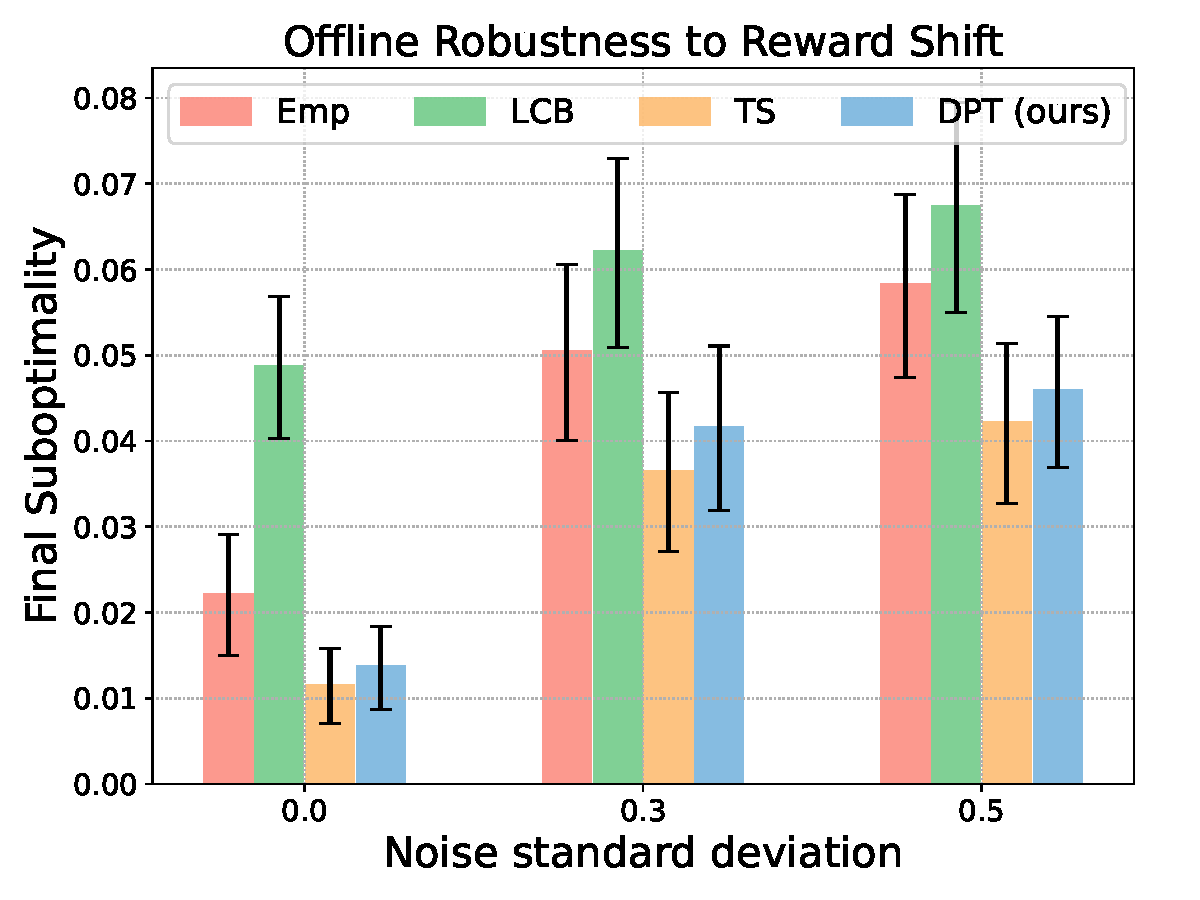
\includegraphics[width=\linewidth]{figures/bandit_offline_vars_epoch300.pdf}
        \caption{}
        \label{fig:vars-offline}
    \end{subfigure}
    \begin{subfigure}{0.32\textwidth}
        \centering
        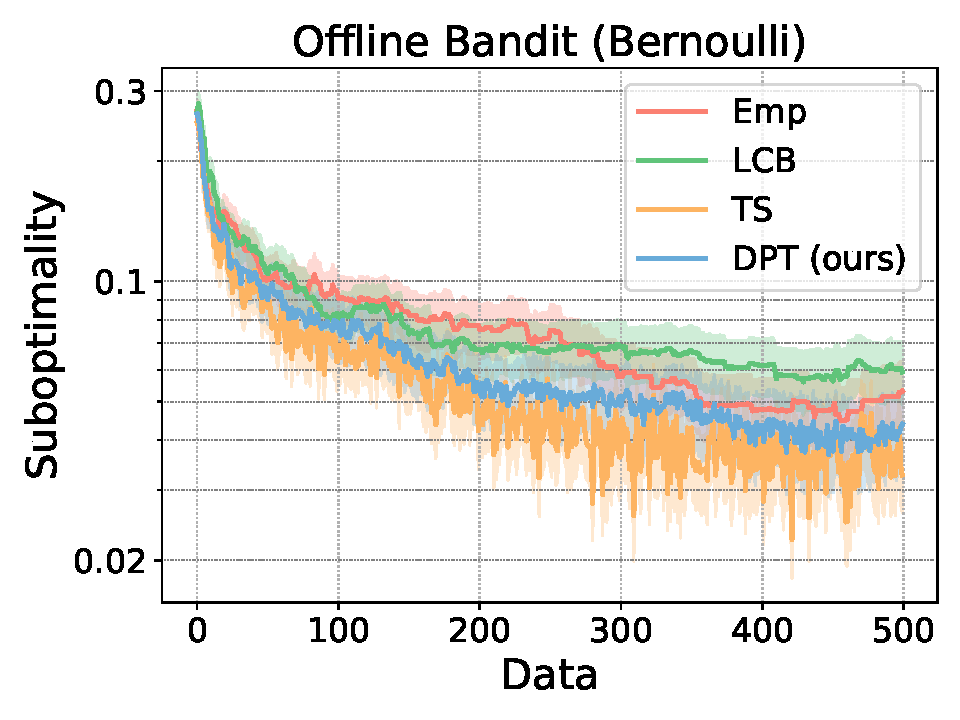
\includegraphics[width=\linewidth]{figures/bernoulli_bandit_offline_epoch300.pdf}
        \caption{}
        \label{fig:bernoulli-offline}
    \end{subfigure}
    \begin{subfigure}{0.32\textwidth}
        \centering
        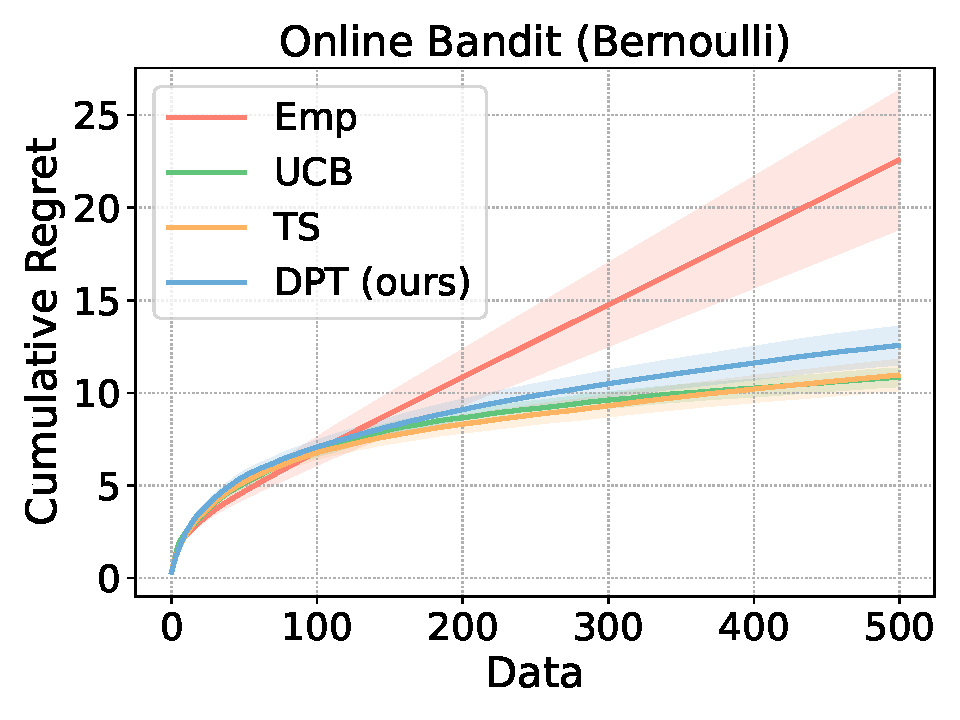
\includegraphics[width=\linewidth]{figures/bernoulli_bandit_online_epoch300.pdf}
        \caption{}
        \label{fig:bernoulli-online}
    \end{subfigure}
    \caption{\small (a) Final (after 500 steps) offline suboptimality on out-of-distribution bandits with different Gaussian noise standard deviations. (b) Offline performance on out-of-distribution Bernoulli bandits, given random in-context datasets. (c) Online cumulative regret on Bernoulli bandits. The mean and standard error are computed over $200$ test tasks.}
    
\end{figure}

\subsection{Bandits}

This section reports additional experimental results in bandit environments.

\paragraph{Out-of-distribution reward variances. } In Figures~\ref{fig:online-vars} and~\ref{fig:vars-offline}, we demonstrate the robustness of the basic pretrained model under shifts in the reward distribution at test time by varying the amount of noise observed in the rewards. \macroName{} maintains robustness to these shifts similar to TS.

\paragraph{Bernoulli rewards.} We test the out-of-distribution ability of \macroName{} further by completely changing the reward distribution from Gaussian to Bernoulli bandits. Despite being trained only on Gaussian tasks during pretraining, \macroName{} maintains strong performance both offline and online in Figures~\ref{fig:bernoulli-offline} and~\ref{fig:bernoulli-online}. 


\begin{wrapfigure}{r}{0.24\textwidth}
  \centering
    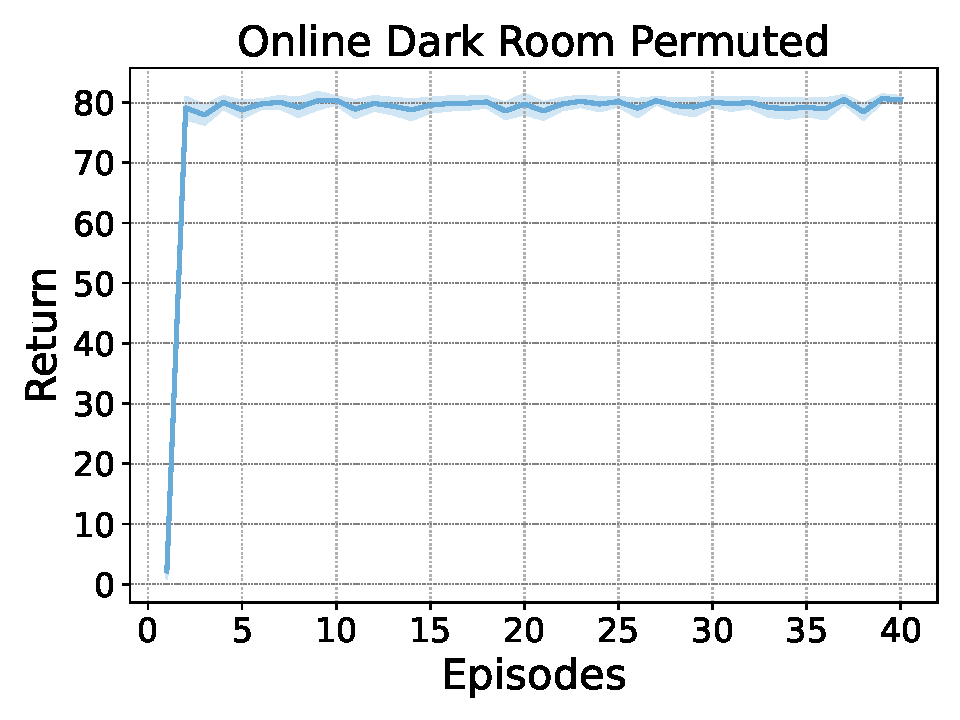
\includegraphics[width=\linewidth]{figures/darkroom_online_permute_trainFalse.pdf}
    \caption{\small Online evaluation of DPT on Dark Room when tested on novel actions set permutations.}
    \label{fig:mdp-permute}
    \vspace{-1cm}
\end{wrapfigure}


\begin{figure}
    \centering
    \begin{subfigure}{0.24\textwidth}
        \centering
        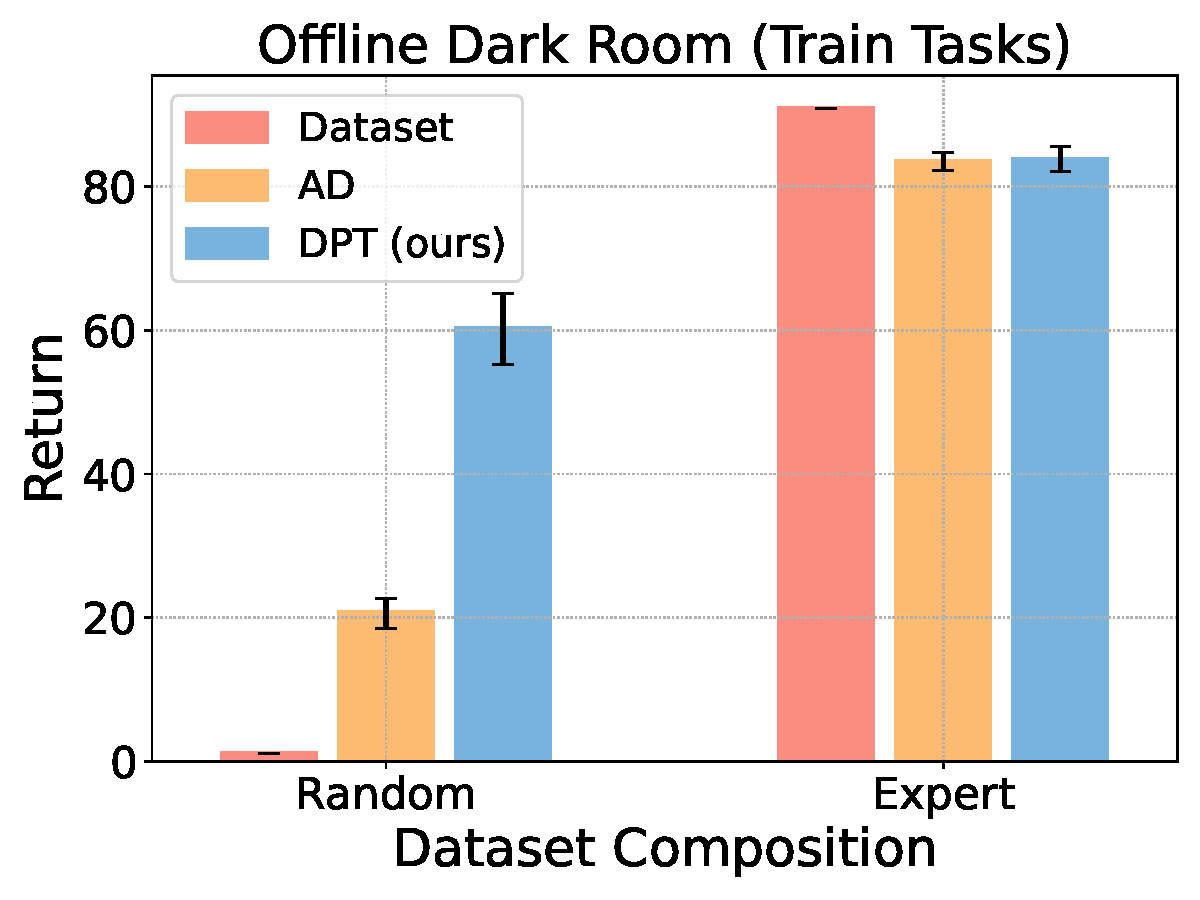
\includegraphics[width=\linewidth]{figures/darkroom_offline_trainTrue.pdf}
        \caption{}
        \label{fig:dark-offline-train}
    \end{subfigure}
    \begin{subfigure}{0.24\textwidth}
        \centering
        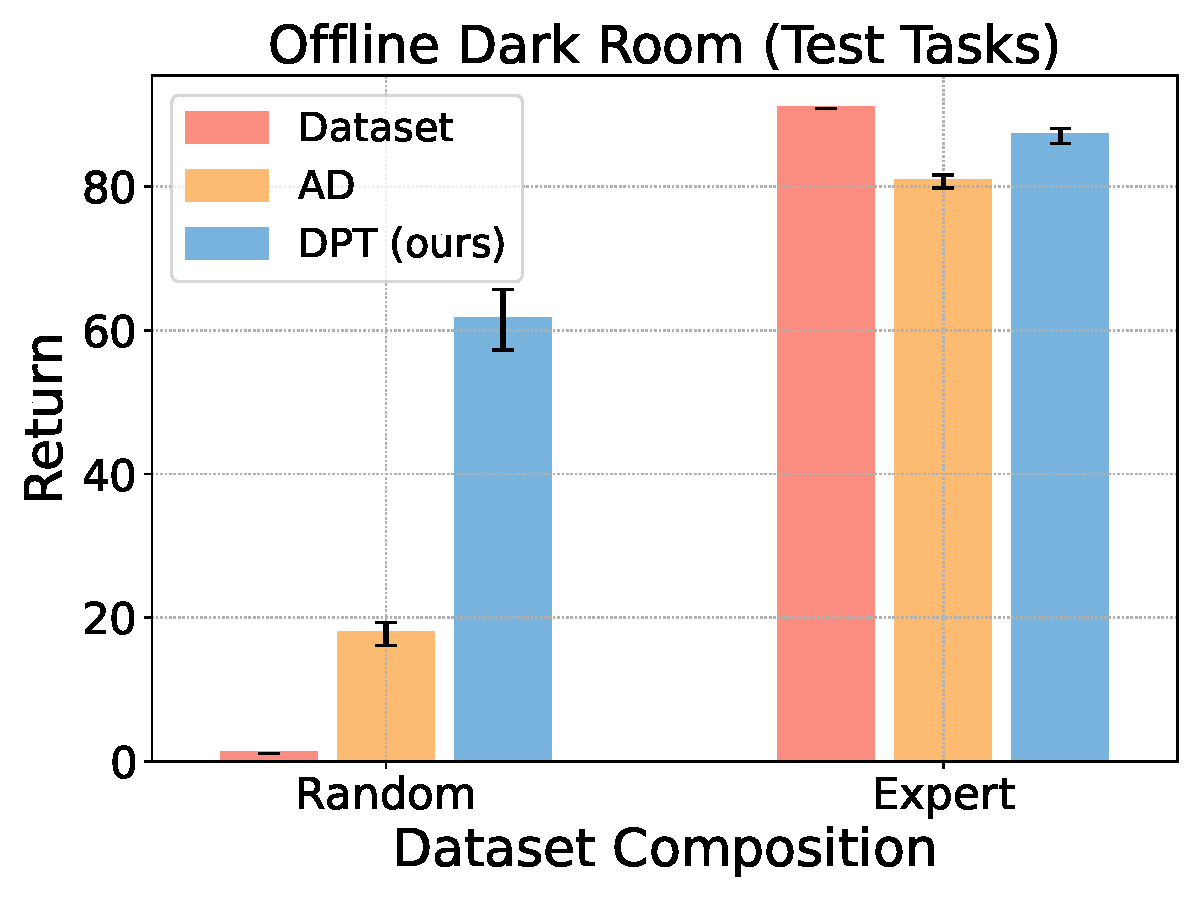
\includegraphics[width=\linewidth]{figures/darkroom_offline.pdf}
        \caption{}
        \label{fig:dark-offline-train2}
    \end{subfigure}
        \begin{subfigure}{0.24\textwidth}
        \centering
        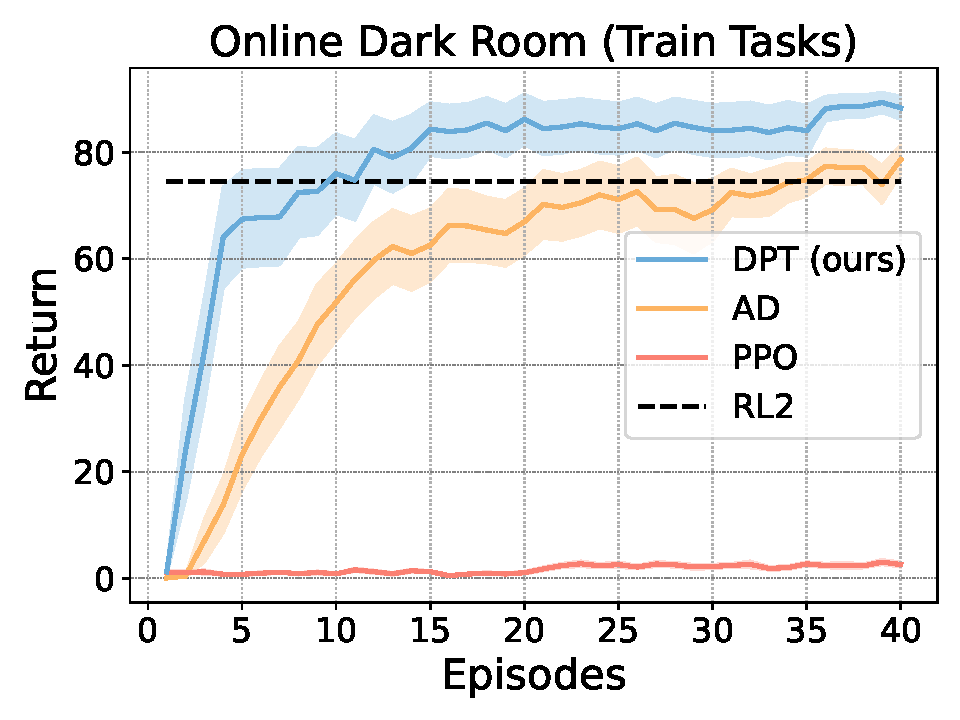
\includegraphics[width=\linewidth]{figures/darkroom_trainTrue.pdf}
        \caption{}
        \label{fig:dark-online-train}
    \end{subfigure}
        \begin{subfigure}{0.24\textwidth}
        \centering
        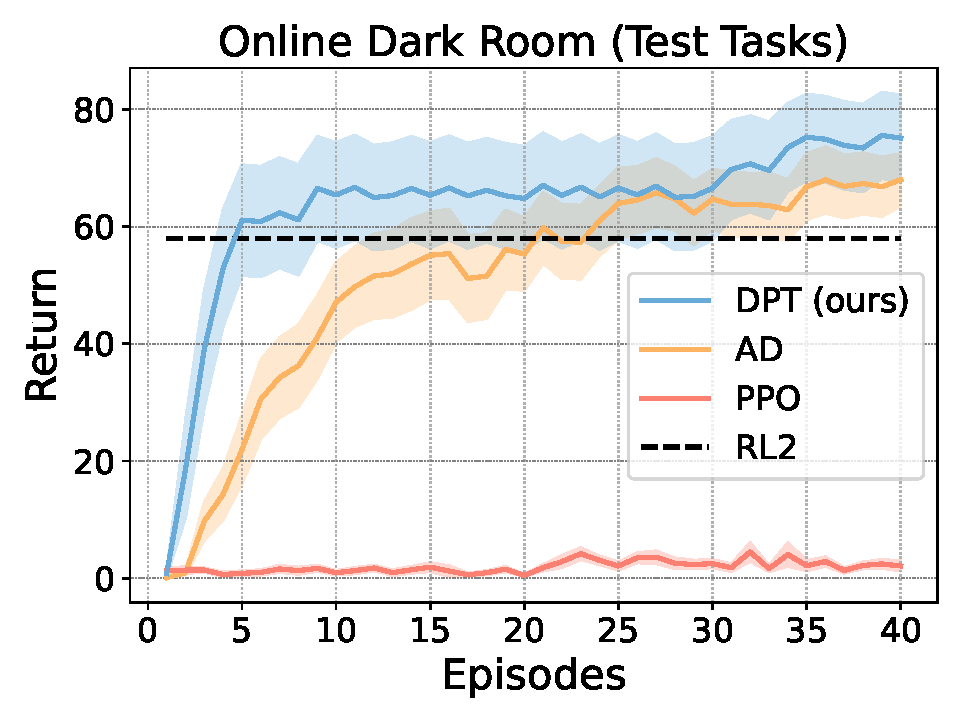
\includegraphics[width=\linewidth]{figures/darkroom_trainFalse.pdf}
        \caption{}
        \label{fig:dark-online-train2}
    \end{subfigure}


    \caption{\small All comparisons in Dark Room evaluated on the tasks that were seen during pretraining, displayed next to their evaluations on test task counterparts from the main text.}
    \label{fig:darkroom-train}
\end{figure}





\subsection{Markov Decision Processes}
This section reports additional experimental results in the Dark Room and Miniworld environments.





\paragraph{Performance on training tasks.} In Fig.~\ref{fig:darkroom-train}, we show the performance of each method on the training tasks in Dark Room. Offline, \macroName{} and AD demonstrate comparable performance as on the training tasks, indicating a minimal generalization gap to new goals. Online, \macroName{}, AD, and RL$^2$ also achieve performance on the training tasks similar to that on the test tasks.



\paragraph{Generalization to new dynamics.} In this experiment, we study generalization to variations in a different aspect of the MDP, namely the dynamics. We design \emph{Dark Room (Permuted)}, a variant of Dark Room in which the goal is fixed to a corner but the action space is randomly permuted. Hence, the agent must leverage its historical context to infer the effect of each action. On a held-out set of $20$ permutations, \macroName{} infers the optimal policy correctly every time offline, given only $100$ offline samples, matching the optimal policy at $83$ return. Similarly, the online performance immediately snaps to a near optimal policy in one episode once it identifies the novel permutation in Figure~\ref{fig:mdp-permute}.









\begin{figure}
    \centering
    \begin{subfigure}{0.24\textwidth}
        \centering
        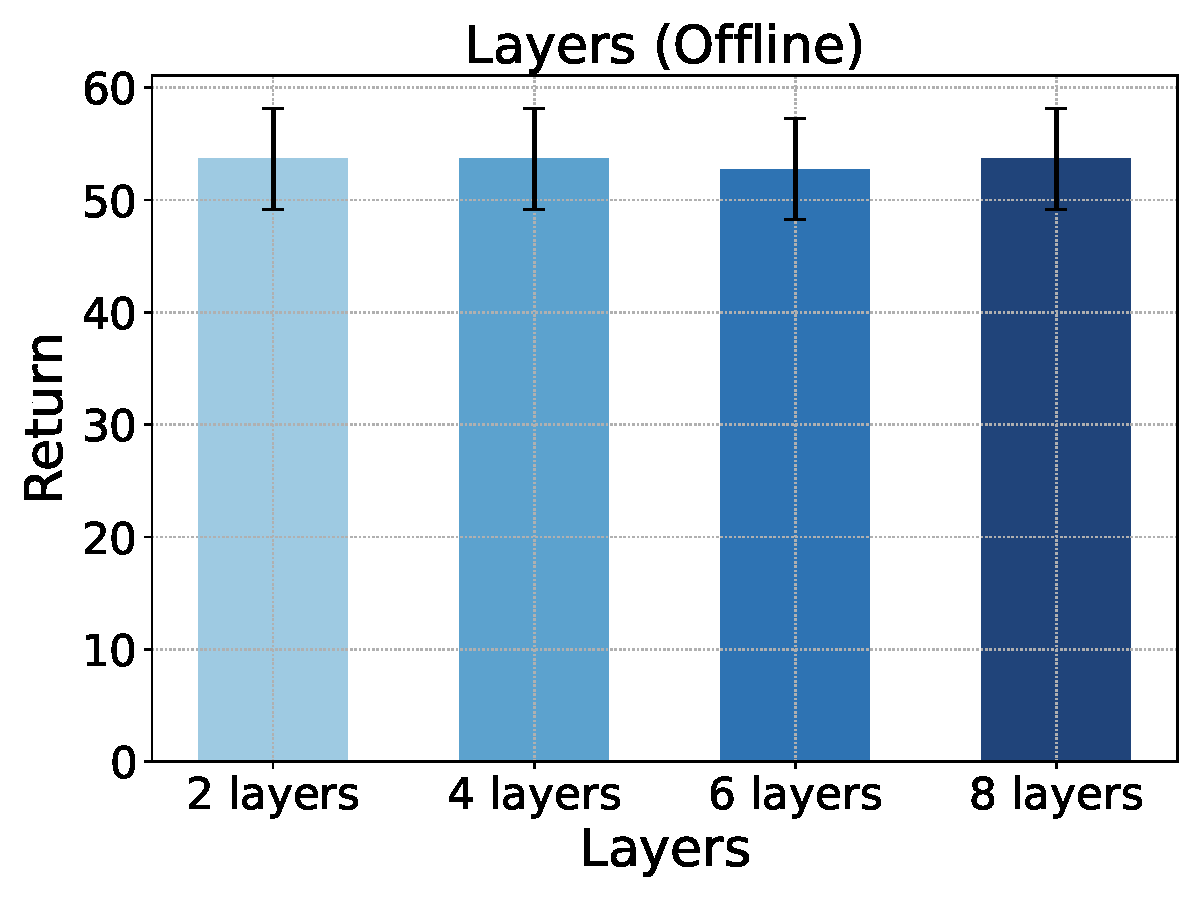
\includegraphics[width=\linewidth]{figures/darkroom_offline_layers.pdf}
        \caption{}
        \label{fig:sens-layers}
    \end{subfigure}
    \begin{subfigure}{0.24\textwidth}
        \centering
        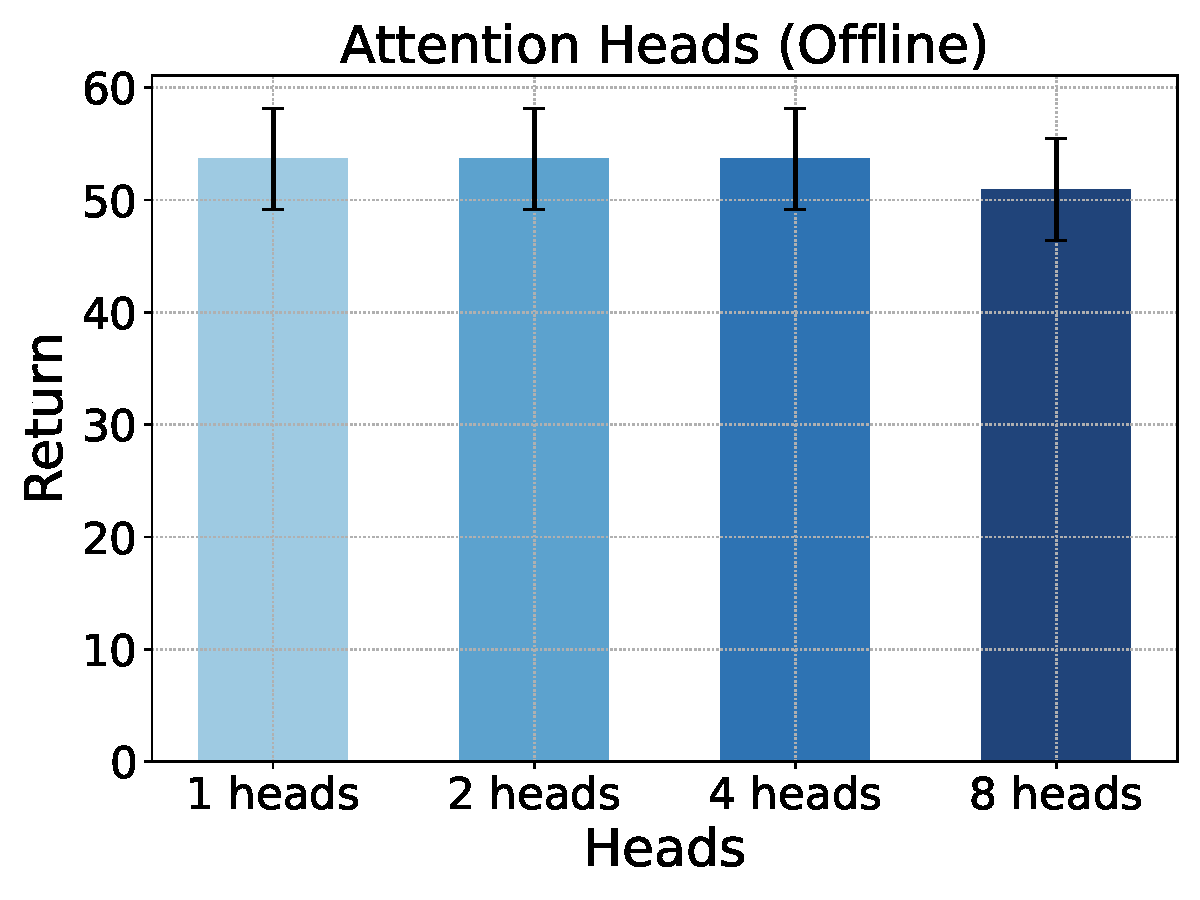
\includegraphics[width=\linewidth]{figures/darkroom_offline_heads.pdf}
        \caption{}
        \label{fig:sens-heads}
    \end{subfigure}
    \begin{subfigure}{0.24\textwidth}
        \centering
        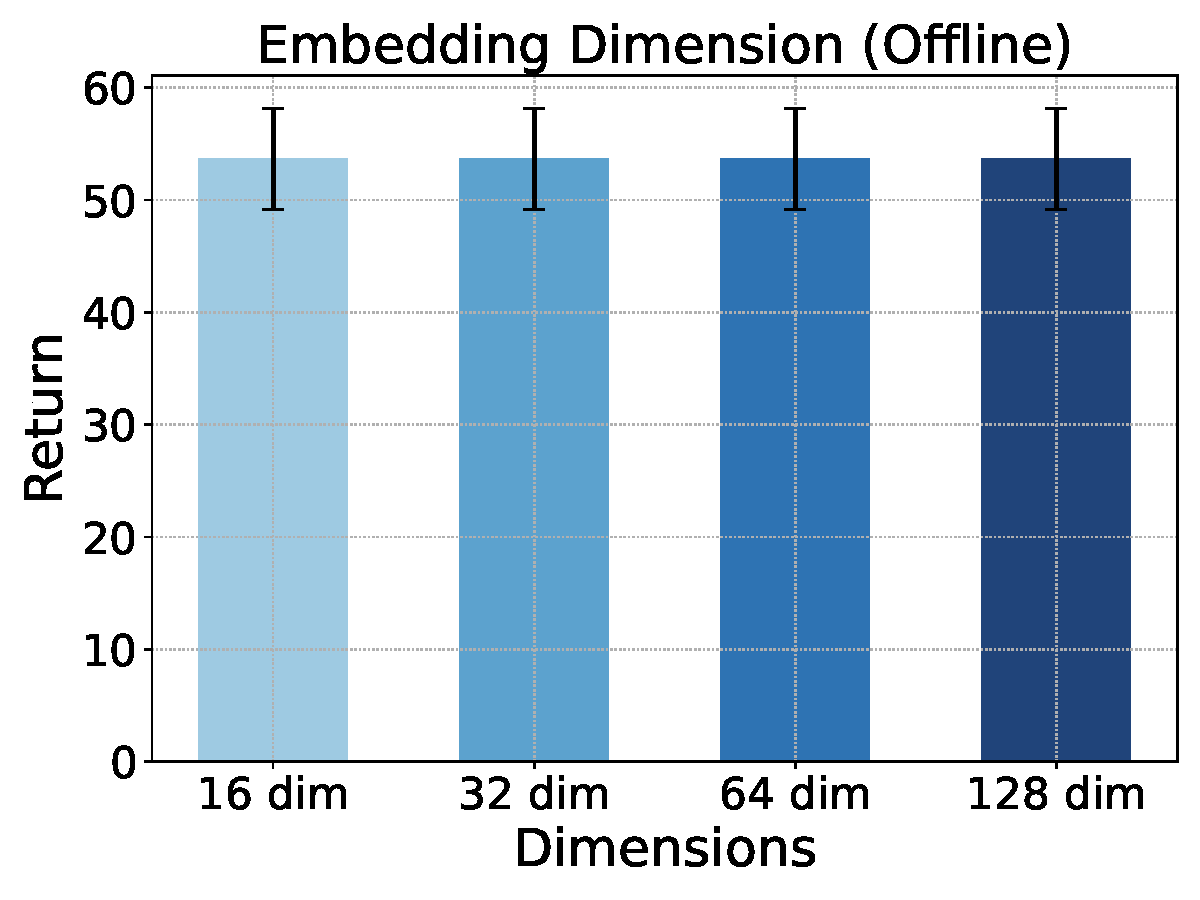
\includegraphics[width=\linewidth]{figures/darkroom_offline_embd.pdf}
        \caption{}
        \label{fig:sens-embd}
    \end{subfigure}
    \begin{subfigure}{0.24\textwidth}
        \centering
        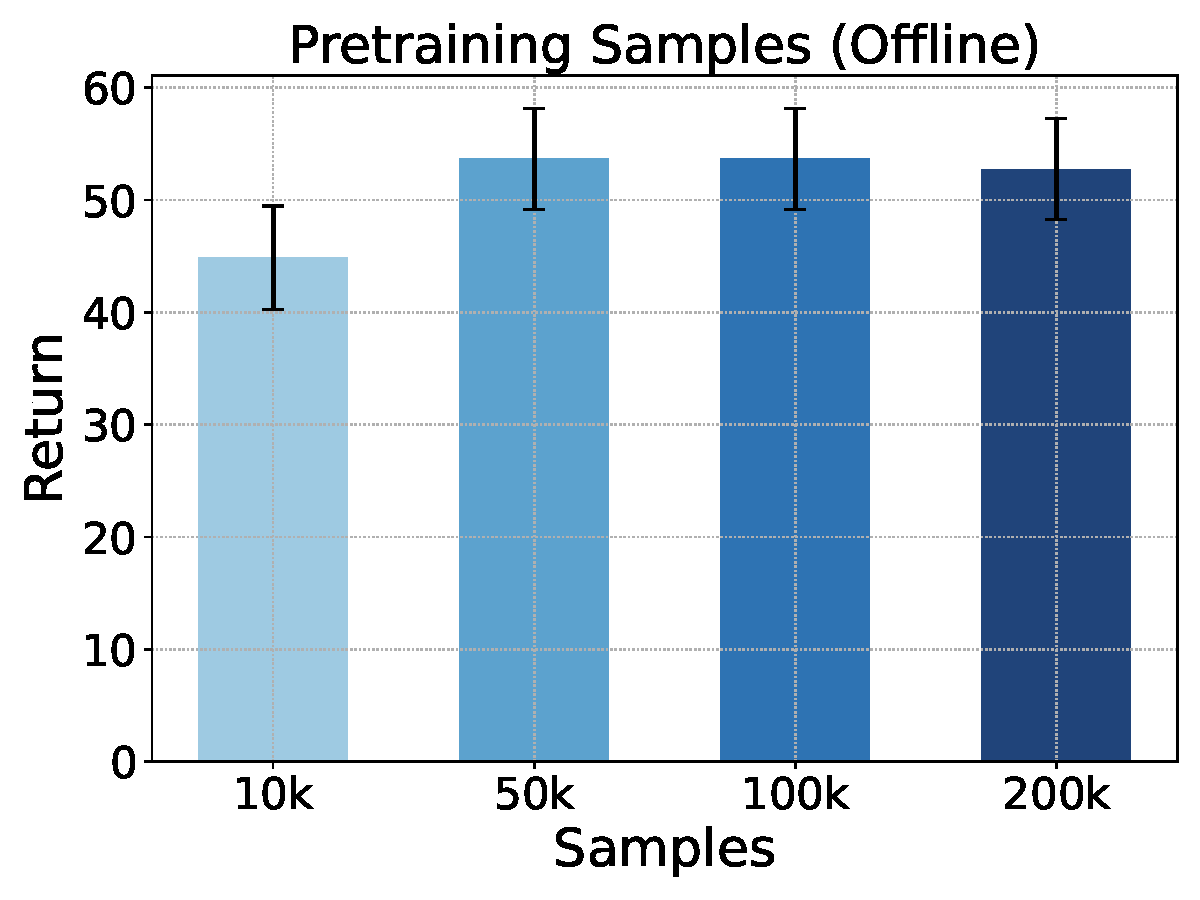
\includegraphics[width=\linewidth]{figures/darkroom_offline_samples.pdf}
        \caption{}
        \label{fig:sens-samples}
    \end{subfigure}
    \caption{\small Sensitivity analysis of the offline Dark Rook task over the GPT-2 transformer's hyperparameters: (a) layers (b) attention  heads (c) embedding dimensions (d) pretraining samples.}
    \label{fig:sensitivity}
\end{figure}


\subsection{Sensitivity Analysis}
We next seek to understand the sensitivity of \macroName{} to different hyperparameters, including the model size and size of the pretraining dataset. These experiments are performed in the Dark Room environment. As shown in Fig.~\ref{fig:sensitivity}, the performance of \macroName{} is robust to the model size; it is the same across different embedding sizes, number of layers, and number of attention heads. Notably, the performance is slightly worse with $8$ attention heads, which may be attributed to slight overfitting. We do see that when the pretraining dataset is reduced to $10\%$ of its original size ($10000$ samples) the performance degrades, but otherwise has similar performance with larger pretraining datasets.








\section{Additional Theory and Omitted Proofs}\label{app:theory}


We start with a well-known concentration inequality for the maximum-likelihood estimate (MLE) to provide some more justification for the approximation made in Assumption~\ref{asmp:equality}. We state a version from~\cite{agarwal2020flambe}.
Let $\Fcal$ be a finite function class used to model a conditional distribution $p_{Y| X} (y | x)$ for $x \in \Xcal$ and $y \in \Ycal$. Assume there is $f^\star \in \Fcal$ such that $p(y | x) = f^\star(y | x)$ (realizable), and $f(\cdot| x) \in \Delta(\Ycal)$ for all $x \in \Xcal$ and $f \in \Fcal$ (proper). Let $D = \{ x_i, y_i\}_{i \in [N]}$ denote a dataset of i.i.d samples where $x_i \sim p_X$ and $y_i \sim p_{Y | X} (\cdot | x_i)$.
Let
\begin{align}
    \hat f = \argmax_{f \in \Fcal}  \sum_{i \in [N]} \log f(y_i | x_i) 
\end{align}
\begin{proposition}[Theorem 21 of~\cite{agarwal2020flambe}]\label{prop:mle}
Let $D$ and $\hat f$ be given as above under the aforementioned conditions. Then, with probability at least $1 - \delta$, 
\begin{align}
    \E_{x \sim p_X}  \| \hat f(\cdot | x) - p_{Y| X}(\cdot | x) \|_1^2 & \leq \frac{8 \log \left( |\Fcal| /\delta \right) }{N}
\end{align}
\end{proposition}
The finiteness of $\Fcal$ is done for simplicity, but we can see that this yields dependence on the log-cardinality,  a common measure of complexity. Extensions to infinite $\Fcal$ of bounded statistical complexity can be readily made to replace this.
For our setting, the bound suggests that $\E_{P_{pre}} \| P_{pre}(\cdot | \squery, D, \xi_h) - M_{\theta} (\cdot | \squery, D, \xi_h) \|_1^2 \rightarrow 0$ as $N \rightarrow \infty$ with high probability, provided the function class of $M_{\theta}$ has bounded statistical complexity.

\subsection{Posterior Sampling}

Posterior sampling is most generally described with the following procedure~\citep{osband2013more}. Initialize a prior distribution $\Tcal_1 = \pretraint$ and dataset $D = \{\}$. For $k \in [K]$
\begin{enumerate}
    \item Sample $\tau_k \sim \Tcal_k$ and compute $\hat \pi_{\tau_k}   $
    \item Execute $\pistar_{\tau_k}$ and add interactions to $D$
    \item Update posterior distribution $\Tcal_{k + 1}(\tau) = P( \tau | D)$.
\end{enumerate}
The prior and posteriors are typically over models such as reward functions in bandits or transition dynamics in MDPs.

\subsection{Proof of Theorem~\ref{thm:main}}

\thmmain*


\begin{proof}
Without loss of generality, for a task $\tau$, we take $\pistar_\tau(\cdot | s)$ to be deterministic and denote the optimal action in state $s$ as $\pistar_\tau(s)$. Recall that we consider a fixed current task $\tau_c$ and a fixed in-context dataset $D$. Define $\xi_{h} = (s_1, a_1, \ldots, s_{h}, a_{h})$.

We now formally state the variant of the full joint distribution from which we sample during pretraining. Let $\tau$ and $D'$ be an arbitrary task and dataset and let $a^\star \in \Acal$, $\squery \in \Scal$, $\xi_{H - 1} \in (\Scal \times \Acal)^{H-1}$, and $h \in [0, H- 1]$ be arbitrary.
\begin{align}
    P_{pre} (\tau, a^\star, \squery, D', \xi_{H - 1}, h) & =  \pretraint(\tau) \pretraind(D'; \tau) \Dquery(\squery)  \Sfrak_H(s_{1:H}) \pistar_\tau(a^\star |\squery)  \\
    & \quad \times \unif{[0, H - 1]} \prod_{i \in [H]} \pistar_\tau( a_i | s_i)
\end{align}
The $\unif[0, H - 1]$ is due to the fact that we sample $h \sim \unif[0, H 
    - 1]$ and then truncate $\xi_h$ from $\xi_{H-1}$ (or, equivalently, sample $\xi_h \sim \Sfrak_h$ directly), marginalizing out the other variables.
For $h' \leq h - 1$, recall that we also use the notation $\Sfrak_{h'}(s_{1:h'})$ to denote the marginalization of the full joint $\Sfrak_H$. We will eventually work with the posterior of this distribution given the data $D$ and history $\xi_h$:
\begin{align}
    P_{pre}(\tau | D, \xi_h) & \propto \pretraint(\tau) \pretraind(D; \tau) \prod_{i \in [h]} \pistar_{\tau}(a_i | s_i) \\
    & \propto P_{pre} (\tau | D) \prod_{i \in [h]} \pistar_{\tau}(a_i | s_i) 
\end{align}


We define the following random sequences and subsequences:
\begin{align}
    \Xi_{ps}(h; D) =  \left(S_1^{ps}, A_1^{ps}, \ldots, S_h^{ps}, A_h^{ps}\right) 
\end{align}
where the variables are generated according to the following conditional process:  $\tau_{ps} \sim P(\cdot | D)$, $S^{ps}_1 \sim \rho_{\tau_c}$, $A^{ps}_h \sim \pistar_{\tau_{ps}}(\cdot | S^{ps}_h)$, and $S_{h + 1}^{ps} \sim T_{\tau_c} (\cdot  | S_{h}^{ps}, A^{ps}_{h}) $. We also define $\Xi_{ps}(h': h; D)$ to be the last $h - h'$ elements of $\Xi_{ps}(h; D)$. Analogously, we define
\begin{align}
    \Xi_{pre}(h; D) =  \left(S_1^{pre}, A_1^{pre}, \ldots, S_h^{pre}, A_h^{pre}\right)
\end{align}
where the variables are from the process: $S_1^{pre} \sim \rho_{\tau_c}$, $A_h^{pre} \sim P_{pre} (\cdot | S_h^{pre}, D, \Xi_{pre}(h - 1; D))$, and $S_{h + 1}^{pre} \sim T_{\tau_c}(\cdot | S_h^{pre}, A_h^{pre})$. Note that $A_h^{pre}$ is sampled conditioned on the sequence $\Xi_{pre}(h; D)$ so far. 

We will show that $\Xi_{ps} (h; D)$ and $\Xi_{pre}(h; D)$ follow the same distribution for all $h \in [H]$. For  convenience, we will drop notational dependence on $D$, except where it resolves ambiguity. Also, because of Assumption~\ref{asmp:equality}, we have that $P_{pre}(\cdot | S^{pre}_h, D, \Xi_{pre}(h - 1)) = M_{\theta} (\cdot | S^{pre}_h, D, \Xi_{pre}(h - 1))$, so we will just work with $P_{pre}$ for the remainder of the proof. We will also make use of the following lemma.
\begin{lemma}\label{lem:compliance}
    If $\pretraind$ is complaint, then $P_{pre} (\tau | D) = P(\tau_{ps} = \tau | D)$.
\end{lemma}
\begin{proof}
From the definition of posterior sampling (using the same prior, $\pretraint$), we have that
    \begin{align}
            P(\tau_{ps}  = \tau | D) & \propto P(D | \tau) \pretraint(\tau) \\
            & \propto \pretraint(\tau) \prod_{j \in [n]} T_{\tau}(s'_j  | s_j, a_j) R_\tau(r_j | s_j, a_j)  \\
            & \propto \pretraint(\tau) \prod_{j \in [n]} T_{\tau}(s'_j  | s_j, a_j) R_\tau(r_j | s_j, a_j) \pretraind(a_j | s_j, D_{j - 1}) \\
            & = \pretraint(\tau) \pretraind(D; \tau) \\
            & = P_{pre}(\tau | D)
    \end{align}
where the second line crucially uses the fact that posterior sampling chooses actions based only on the prior and history so far. Similarly, the third line uses the fact that $\pretraind$ is compliant. Since the two sides are proportional in $\tau$, they are equivalent.
\end{proof}



We will prove Theorem~\ref{thm:main} via induction for each $h \in [H]$. First, consider the base case for a sequence of length $h = 1$. Recall that $\rho_{\tau_c}$ denotes the initial state distribution of $\tau_c$. We have that the densities can be written as
\begin{align}
    P(\Xi_{ps}(1) = \xi_1) &  = P(S^{ps}_1  = s_1, A^{ps}_1 = a_1) \\
    & = \rho_{\tau_c}(s_1) P(A^{ps}_1 = a_1 | S^{ps}_1 = s_1) \\
    & = \rho_{\tau_c}(s_1) \int_{\tau} P(A^{ps}_1 = a_1, \tau_{ps} = \tau | S^{ps}_1 = s_1) d\tau \\
    & = \rho_{\tau_c}(s_1) \int_{\tau} \pistar_\tau(a_1 | s_1)  P_{ps} (\tau_{ps} = \tau | D, S^{ps}_1 = s_1) d\tau \\
    & = \rho_{\tau_c}(s_1) \int_{\tau} \pistar_\tau(a_1 | s_1)  P_{ps} (\tau_{ps} = \tau | D) d\tau \\
    & = \rho_{\tau_c}(s_1) P_{pre}( A^{pre}_1 = a_1 | s_1, D) \\
    & = P(\Xi_{pre}(1) = \xi_1)
\end{align}
where the second line uses the sampling process of $S^{pre}_1$; the third marginalizes over $\tau_{ps}$, which is the task that posterior sampling samples to find the optimal policy; the fourth decomposes this into the optimal policy and the posterior over $\tau_{ps}$ given $D$ and $S^{ps}_1$. Since $S^{ps}_1$ is independent of sampling of $\tau_{ps}$ this dependence goes away in the next line. The sixth line applies Lemma~\ref{lem:compliance} and then, for $h = 1$, there is no history to condition on.

Now, we leverage the inductive hypothesis to prove the full statement. Suppose that the hypothesis holds for $h - 1$. Then, 
\begin{align}
    P(\Xi_{ps}(h) = \xi_h) & = P(\Xi_{ps}(h - 1) = \xi_{h - 1})  P(S^{ps}_{h} = s_h, A^{ps}_h = a_h | \Xi_{ps}(h - 1) = \xi_{h - 1}) \\
\end{align}
By the hypothesis, we have that $P(\Xi_{ps}(h - 1) = \xi_{h - 1}) = P(\Xi_{pre}(h - 1) = \xi_{h - 1}) $.  For the second factor,
\begin{align}
     & P(S^{ps}_{h} = s_h, A^{ps}_h = a_h | \Xi_{ps}(h - 1) = \xi_{h - 1}) \\
     & = T_{\tau_c} ( s_h | s_{h - 1},  a_{h - 1})  \cdot P(A_h^{ps} = a_h | S^{ps}_h = s_h, \Xi_{ps}(h - 1) = \xi_{h - 1})\\
     % & = T_{\tau_c} ( s_h |  s_{h - 1},  a_{h - 1}) \cdot  P(A_h^{ps} = a_h | S^{ps}_h = s_h, \Xi_{ps}(h - 1) = \xi_{h - 1}) \\
      & = T_{\tau_c} (s_h |  s_{h - 1}, a_{h - 1}) \cdot  \int_{\tau} P(A_h^{ps} = a_h, \tau_{ps} = \tau | S^{ps}_h = s_h, \Xi_{ps}(h - 1) = \xi_{h - 1}) d\tau
\end{align}
As before, we can further rewrite the last factor as
\begin{align}
    & P(A_h^{ps} = a_h, \tau_{ps} = \tau | S^{ps}_h = s_h, \Xi_{ps}(h - 1) = \xi_{h - 1}) \\
    & = \pistar_{\tau}(a_h | s_h) \cdot P(\tau_{ps} = \tau  |  S^{ps}_h = s_h,  \Xi_{ps}(h - 1) = \xi_{h - 1})
\end{align}
where
\begin{align}
    P(\tau_{ps} = \tau  |  S^{ps}_h = s_h,  \Xi_{ps}(h - 1) = \xi_{h - 1}) 
    & = \frac{P(S^{ps}_h = s_h, \Xi_{ps}(h - 1) = \xi_{h - 1 }  | \tau_{ps} = \tau ) P(\tau_{ps} = \tau | D) } {P(S^{ps}_h = s_h, \Xi_{ps}(h - 1) = \xi_{h - 1 } )} \\
    & \propto P_{pre}(\tau | D)\prod_{i \in [h - 1]} T_{\tau_c} ( s_{i + 1} | s_i, a_i)  \pistar_{\tau}(a_i | s_i) \\
    & \propto P_{pre}(\tau | D)\prod_{i \in [h - 1]} \pistar_{\tau}(a_i | s_i) \\
    & \propto P_{pre}(\tau | D) \Dquery(s_h) \Sfrak_{h - 1} (s_{1:h - 1}) \prod_{i \in [h - 1]}  \pistar_{\tau}(a_i | s_i) \\
    & \propto P_{pre}(\tau | s_h, D, \xi_{h - 1})  \\
\end{align}
where $\propto$ denotes that the two sides are equal up to multiplicative factors independent of $\tau$.  In the first line, we used Bayes rule. In the second line, given that $\tau_{ps} = \tau$ (i.e. posterior sampling selected $\tau$ to deploy),  we decompose the probability of observing that sequence of states of actions. We also used Lemma~\ref{lem:compliance}. The denominator does not depend on $\tau$. Similarly, for the third and fourth lines, $T_{\tau_c}$ and $\Sfrak$ do not depend on $\tau$. The final line follows from the definition of the joint pretraining distribution in this regime.


Therefore, we conclude that the posterior over the value of $\tau_{ps}$ is the same as the posterior over the task in the pretraining distribution, given $s_h, D, \xi_{h - 1}$. Substituting back through all the previous equations, we have
\begin{align}
    & P(\Xi_{ps}(h) = \xi_h) \\
    & = P(\Xi_{pre}(h - 1) = \xi_{h - 1} ) \cdot T_{\tau_c}(s_h | s_{h - 1}, a_{h - 1})\int_{\tau} \pistar_\tau(a_h| s_h) P_{pre}(\tau | s_h, D, \xi_{h - 1}) d \tau \\
    & = P(\Xi_{pre}(h - 1) = \xi_{h - 1} ) \cdot T_{\tau_c}(s_h | s_{h - 1}, a_{h - 1}) P_{pre}(a_h | s_h, D, \xi_{h - 1}) \\
    & = P(\Xi_{pre}(h) = \xi_h)
\end{align}
This concludes the proof.



     
   
\end{proof}












\subsection{Proof of Corollary~\ref{cor:mdp}}

\cormdp*

\begin{proof} Note that $\pretraind$ is clearly compliant since it is generated by random sampling.
We use the equivalence between $M_{\theta}$ and posterior sampling established in Theorem~\ref{thm:main}.
The proof then follows immediately from Theorem~1 of \cite{osband2013more} to guarantee that
\begin{align}
    \E_{\pretraint} \left[ \regret_\tau(M_{\theta})\right] & \leq \widetilde{\Ocal} \left(H^{3/2}S\sqrt{A K}\right)
\end{align}
where the notation $\widetilde{\Ocal}$ omits polylogarithmic dependence. The bound on the test task distribution follows from the assumed bound on the likelihood ratio under the priors:
\begin{align}
     \int \testt(\tau) \regret_\tau(M_{\theta})  d\tau  & \leq  \Ccal \int \pretraint(\tau) \regret_\tau(M_{\theta})  d\tau.
\end{align}
\end{proof}

\subsection{Proof of Corollary~\ref{cor:lin}}

\corlin*

\begin{proof}
    The distribution $\pretraind$ satisfies compliance by definition because it is generated by an adaptive algorithm TS.
    The proof once again follows by immediately deferring  to the established result of \cite{russo2014learning} (Proposition~3) for linear bandits by the posterior sampling equivalence of Theorem~\ref{thm:main}. This ensures that posterior sampling achieves regret $\widetilde{\Ocal}(d\sqrt{K})$. It remains, however, to justify that $P_{pre}(\cdot | D_k)$ will be covered by Gaussian Thompson Sampling for all $D_k$ with $k \in [K]$. This is verified by noting that $P_{ps}(a | D_k) > 0$ for non-degenerate Gaussian Thompson Sampling (positive variances of the prior and likelihood functions) and finite $K$. This guarantees that any $D_k$ will have support.
\end{proof}



\subsection{Proof of Proposition~\ref{prop:invariance}}

\propinvariance*

\begin{proof}
    The proof follows by direct inspection of the pretraining distributions. For $P^1_{pre}$, we have
    \begin{align}
         P^1_{pre} ( a^\star | \squery, D, \xi) & = \int_{\tau} \pistar_\tau(a^\star | \squery) P^1_{pre}(\tau| \squery, D, \xi) d \tau \label{eqn:invariant_tau}
    \end{align}
    The posterior distribution over tasks is simply
    \begin{align}
     P^1_{pre}(\tau| \squery, D, \xi) & = \frac{P^1_{pre}(\tau, \squery, D, \xi)}{P^1_{pre}(\squery, D, \xi)} \\
     & \propto P^1_{pre}(\tau) P^1_{pre} (\xi | \tau)  \Dquery(\squery) \pretraind^1 (D ; \tau) \\
     & = P^2_{pre}(\tau) P^2_{pre} (\xi | \tau)  \Dquery(\squery) \pretraind^1 (D ; \tau)
    \end{align}
    Then, the distribution over the in-context dataset can be decomposed as
    \begin{align}
        \Dcal^1_{pre} (D ; \tau) & = \prod_{i \in [n]} R_\tau(r_i | s_i, a_i) T_\tau(s'_i | s_i, a_i) \pretraind^1( a_i | s_i, D_{i - 1}; \tau) \\
        & = \prod_{i \in [n]} R_\tau(r_i | s_i, a_i) T_\tau(s'_i | s_i, a_i) \pretraind^1( a_i | s_i, D_{i - 1}) \\
        & \propto \prod_{i \in [n]} R_\tau(r_i | s_i, a_i) T_\tau(s'_i | s_i, a_i) \pretraind^2( a_i | s_i, D_{i - 1}) \\ %\frac{\pretraind^2( a_i | s_i, D_{i - 1})}{\pretraind^2( a_i | s_i, D_{i - 1})} \\
        % & = \prod_{i \in [n]} R_\tau(r_i | s_i, a_i) T_\tau(s'_i | s_i, a_i) \pretraind^2( a_i | s_i, D_{i - 1}) \prod_{i \in [n]} \frac{\pretraind^1( a_i | s_i, D_{i - 1})}{\pretraind^2( a_i | s_i, D_{i - 1})} \\
        % & = \prod_{i \in [n]} R_\tau(r_i | s_i, a_i) T_\tau(s'_i | s_i, a_i) \pretraind^2( a_i | s_i, D_{i - 1},\tau) \prod_{i \in [n]} \frac{\pretraind^1( a_i | s_i, D_{i - 1})}{\pretraind^2( a_i | s_i, D_{i - 1})} \\        
    %    & \propto \prod_{i \in [n]} R_\tau(r_i | s_i, a_i) T_\tau(s'_i | s_i, a_i) \\
        & =  \Dcal^2_{pre} (D ; \tau),
    \end{align}
    where the second equality holds because $\pretraind^1(a_j|s_j,D_j; \tau)$ is assumed to be invariant to $\tau$ by compliance, and the fifth equality holds because $\pretraind^2(a_j|s_j,D_j; \tau)$ is assumed to be invariant to $\tau$. 
    
    Therefore, we conclude that, for any $s, D, \xi$,
    \begin{align}
        P^1_{pre}(\tau| s, D, \xi) & \propto P^2_{pre}(\tau) P^2_{pre} (\xi | \tau)  \Dquery(s) \pretraind^2 (D ; \tau) \\
        & \propto P^2_{pre}(\tau| s, D, \xi). 
    \end{align}
    Since also $\int_{\tau} P^1_{pre}(\tau| s, D, \xi) = 1 = \int_{\tau} P^2_{pre}(\tau| s, D, \xi) $, then 
    \begin{align}
P^1_{pre}(\tau| s, D, \xi) =  P^2_{pre}(\tau| s, D, \xi).
\end{align}
    
    Substituting this back into Equation\ref{eqn:invariant_tau} yields $P^1_{pre} ( a^\star | s, D, \xi) = P^1_{pre} ( a^\star | s, D, \xi)$.
\end{proof}




